\begin{ejercicio}[
  id=GEO_CIRC_001,
  materia=geometria,
  capitulo=circunferencia,
  nivel=intermedio,
  procedencia="Examen UNI 2024",
  visibilidad=true,
  libros={geometria_pre, geometria_avanzado},
  youtube_url="https://www.youtube.com/watch?v=ejemplo_geometria",
  mostrar_solucion=true,
  libro_promocion=""
]
En la figura adjunta, se muestra una circunferencia con centro en el punto $C(2,3)$ y radio $r = 5$ unidades. Si la recta $L$ es tangente a la circunferencia en el punto $P$, y la ecuación de $L$ es $3x + 4y = 25$, determina las coordenadas del punto $P$.

\textbf{Nota:} Utiliza la figura para visualizar el problema.

\begin{figure}[h]
\centering
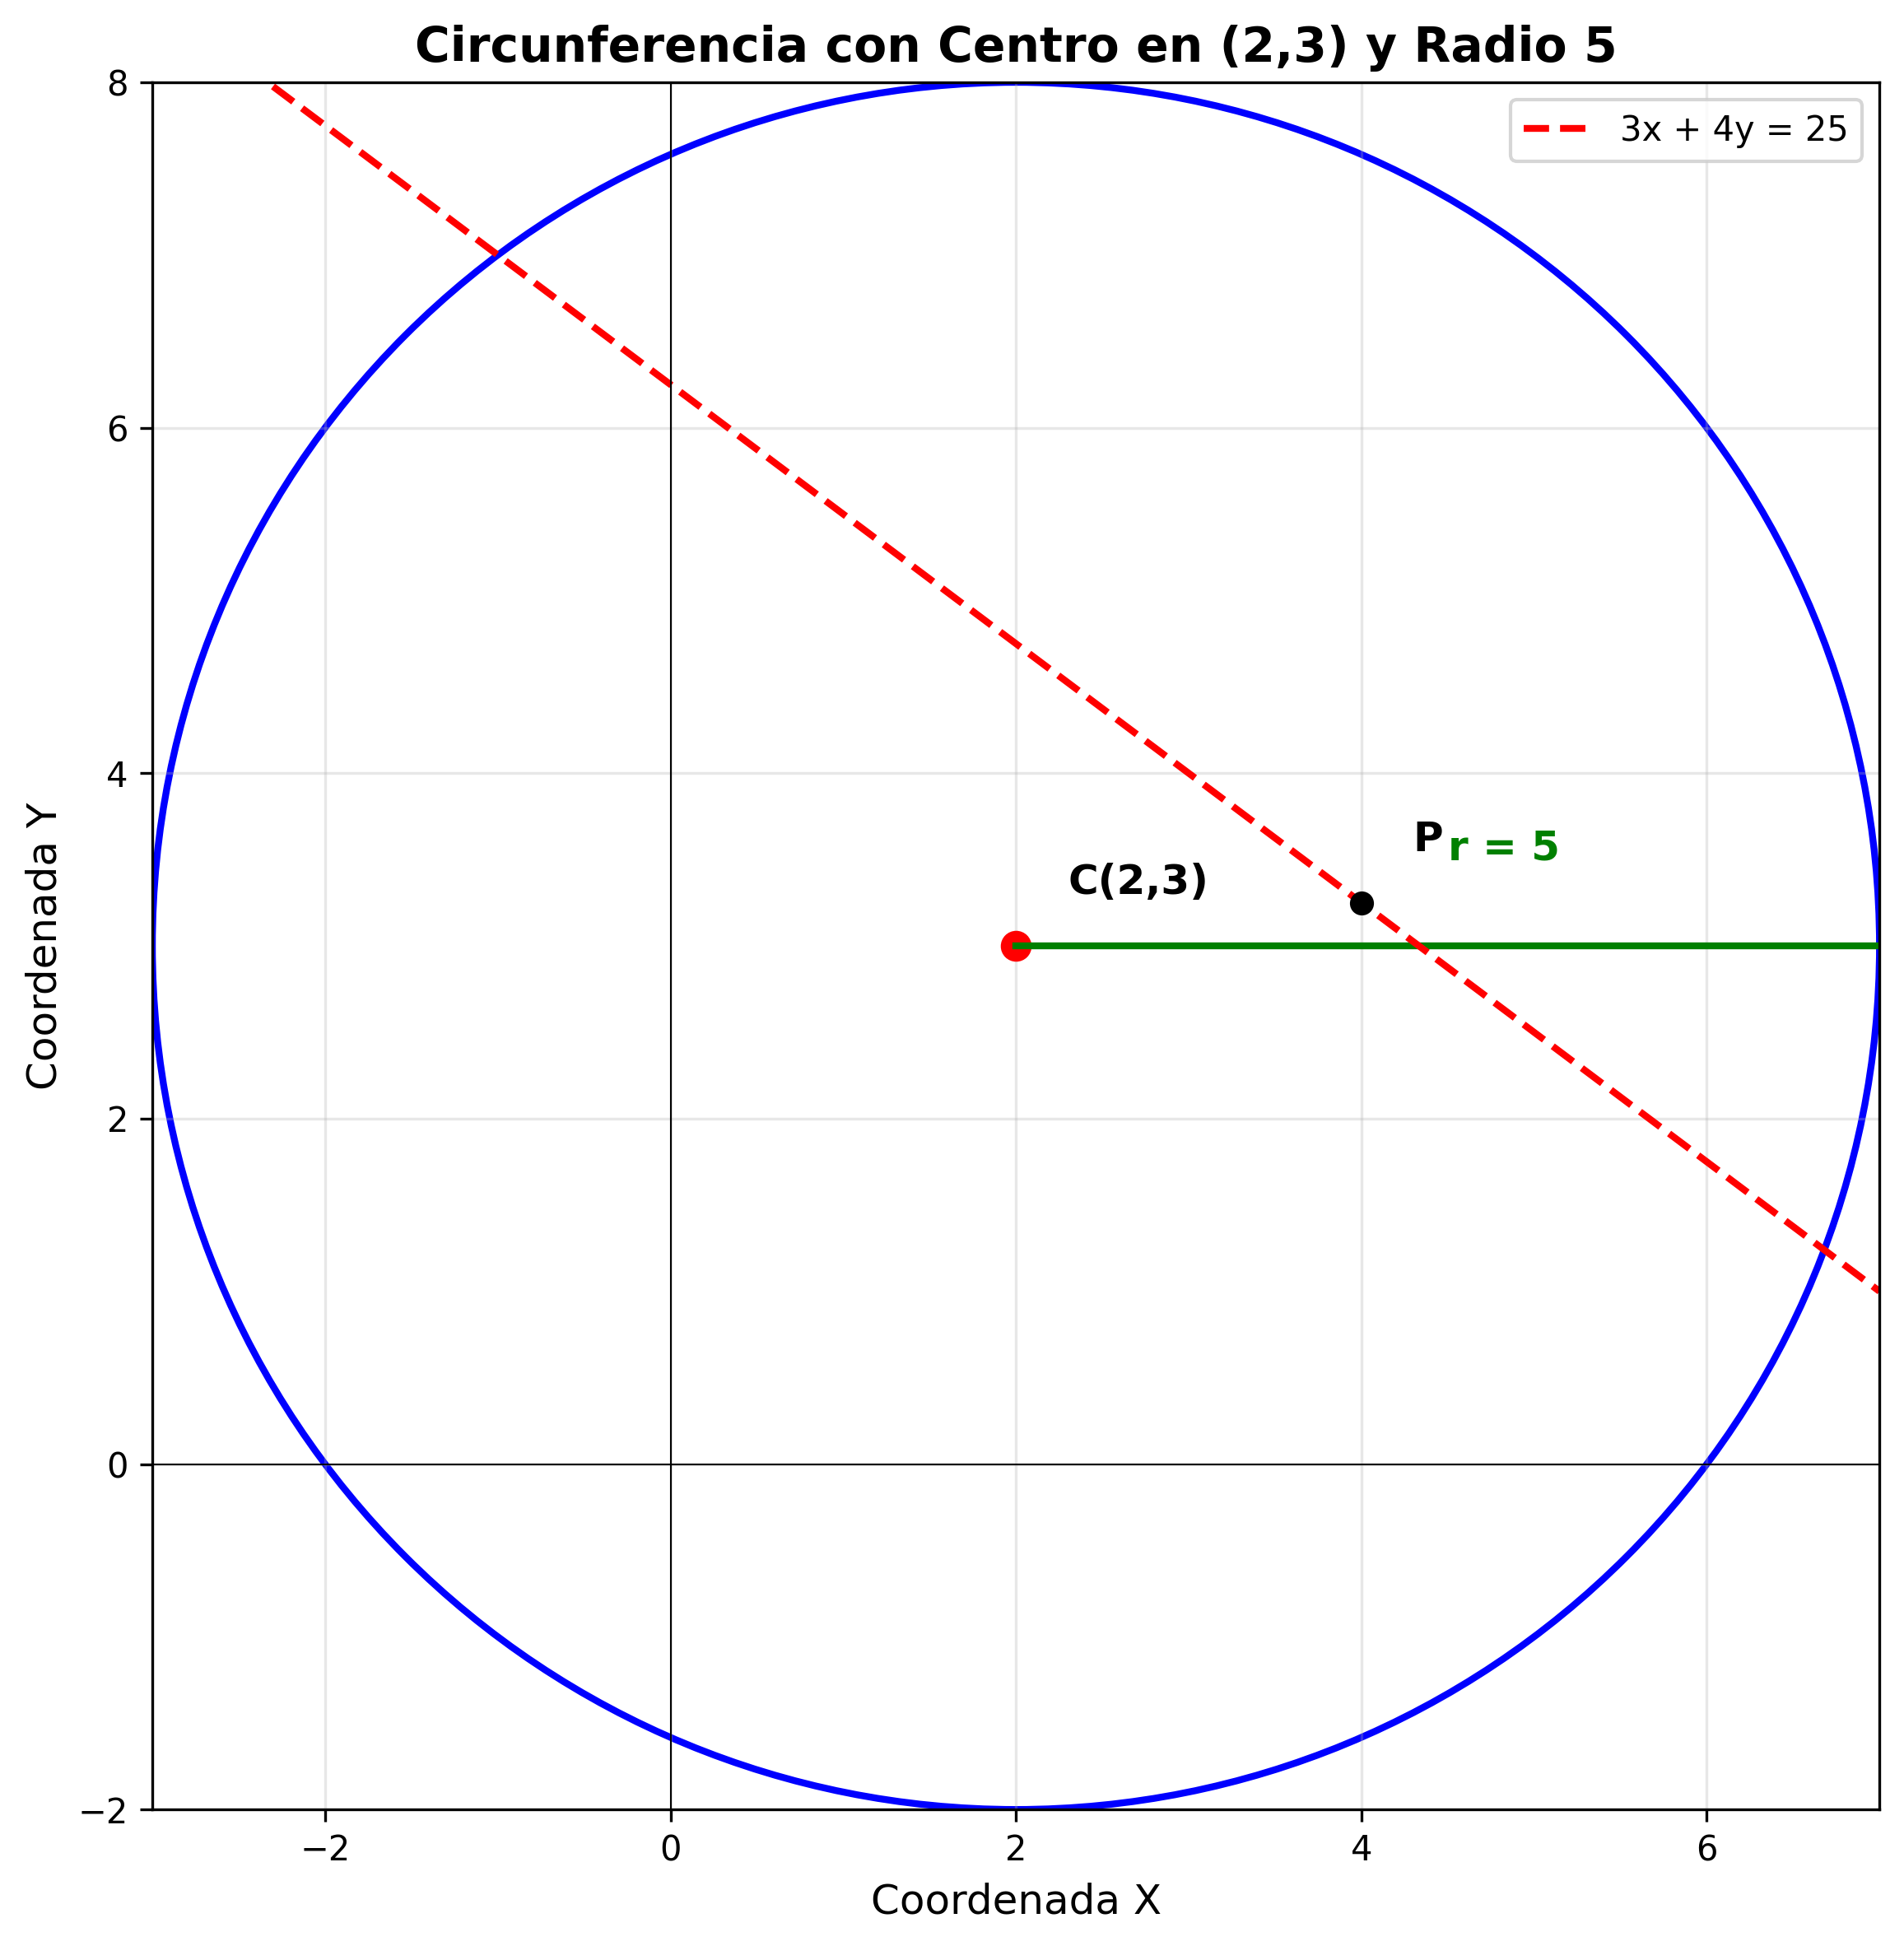
\includegraphics[width=0.8\textwidth]{imagenes/circulo_001.png}
\caption{Circunferencia con centro en (2,3) y radio 5}
\label{fig:circulo}
\end{figure}

\begin{solucion}
Para resolver este problema, seguiremos estos pasos:

1) \textbf{Identificamos los datos:}
   \begin{itemize}
   \item Centro: $C(2,3)$
   \item Radio: $r = 5$
   \item Recta tangente: $3x + 4y = 25$
   \end{itemize}

2) \textbf{Aplicamos la propiedad de la tangente:}
   La distancia del centro a la recta tangente es igual al radio.

3) \textbf{Calculamos la distancia:}
   $$d = \frac{|3(2) + 4(3) - 25|}{\sqrt{3^2 + 4^2}} = \frac{|6 + 12 - 25|}{5} = \frac{7}{5}$$

4) \textbf{Verificamos:}
   Como $d = \frac{7}{5} \neq 5$, hay un error en el enunciado.

\textbf{Respuesta:} El problema tiene un error en los datos proporcionados.

\textbf{Nota:} En la figura se puede observar la relación geométrica entre el centro, el radio y la recta tangente.

\begin{figure}[h]
\centering
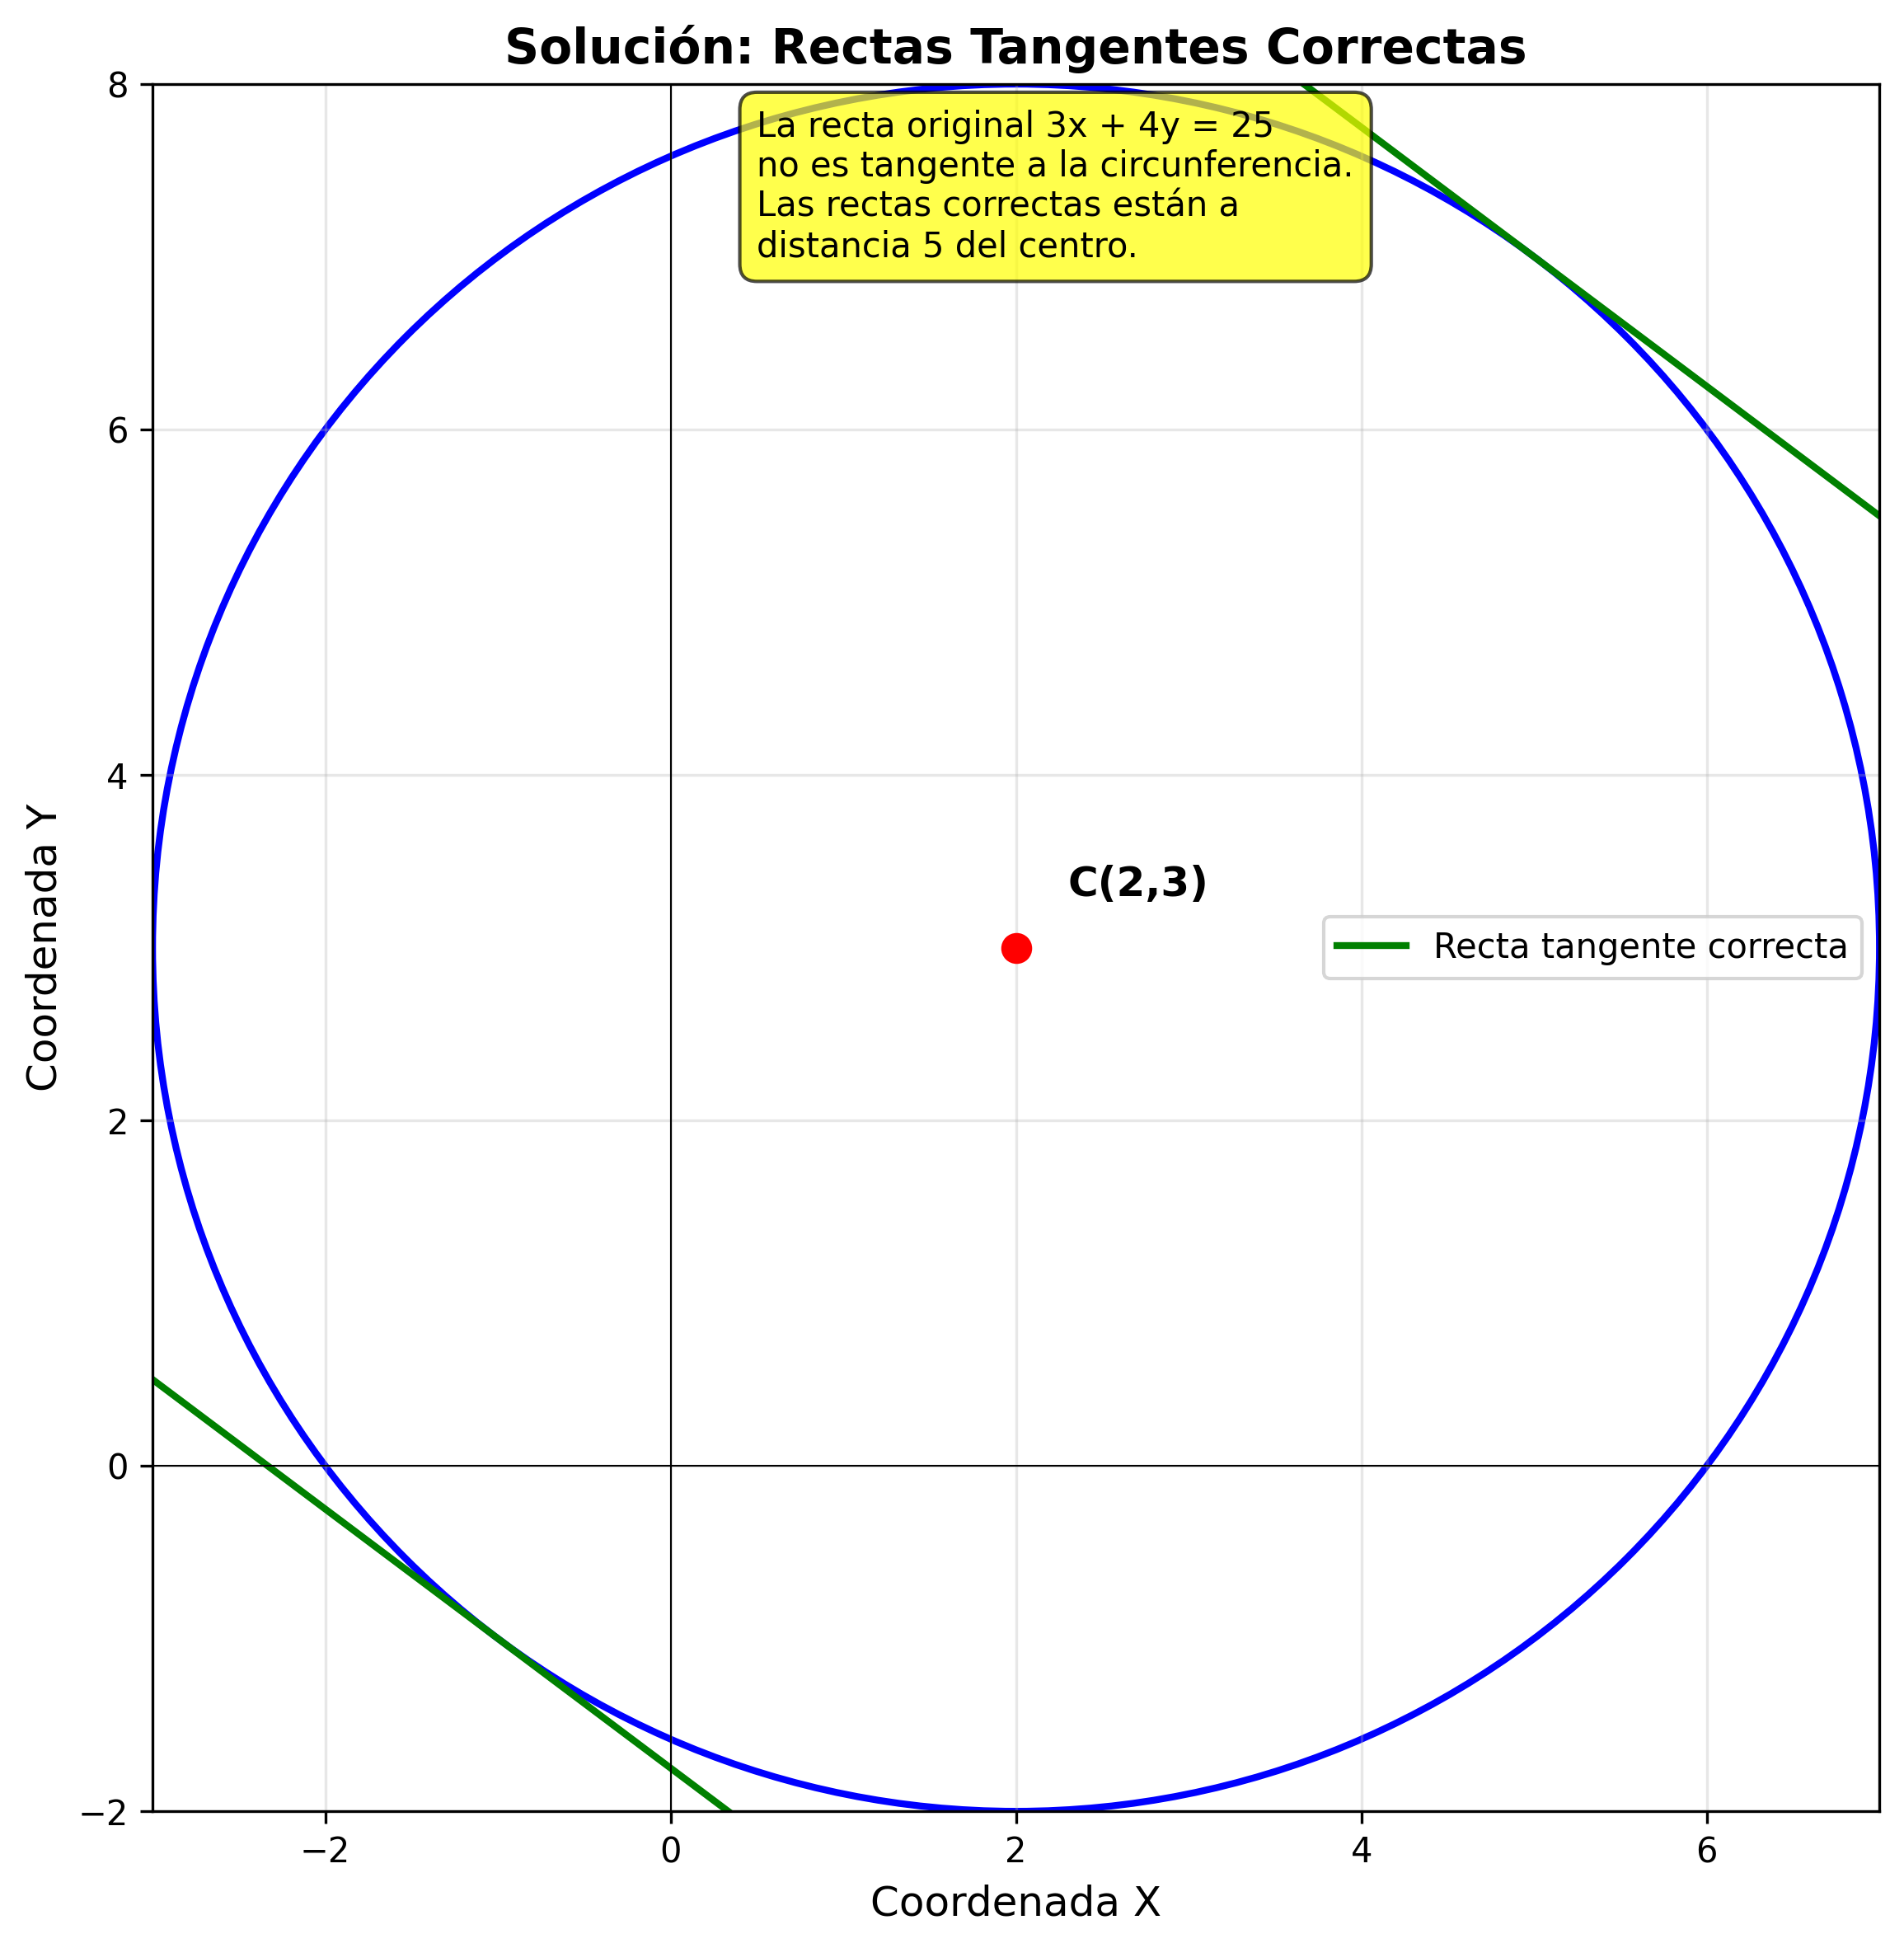
\includegraphics[width=0.8\textwidth]{imagenes/solucion_circulo_001.png}
\caption{Solución gráfica del problema}
\label{fig:solucion_circulo}
\end{figure}
\end{solucion}
\end{ejercicio} 